\chapter{Least Squares Problems} 

Least squares data-fitting has been an indispensable tool since its invention by Gauss and Legendre around 1800, with ramifications extending throughout the mathematical sciences. In the language of linear algebra, the problem here is the solution of an overdetermined system of equations $A x=b$-rectangular, with more rows than columns. The least squares idea is to "solve" such a system by minimizing the 2 -norm of the residual $b-A x$. 

\section{The Problem}
Consider a linear system of equations having $n$ unknowns but $m>n$ equations. Symbolically, we wish to find a vector $x \in \mathbb{C}^n$ that satisfies $A x=b$, where $A \in \mathbb{C}^{m \times n}$ and $b \in \mathbb{C}^m$. 

In general, such a problem has no solution. A suitable vector $x$ exists only if $b$ lies in range $(A)$, and since $b$ is an $m$-vector, whereas range $(A)$ is of dimension at most $n$, this is true only for exceptional choices of $b$. We say that a rectangular system of equations with $m>n$ is \textbf{overdetermined}. The vector known as the \textbf{residual},
$$
r=b-A x \in \mathbb{C}^m
$$
can perhaps be made quite small by a suitable choice of $x$, but in general it cannot be made equal to zero. 

However, we can try to minimize the norm of $r$. If we take the 2-norm, the problem is: 
\begin{equation}
    \label{eq: least sq}
        \min_{x\in \CC^n} \quad \|b-Ax\|_2
\end{equation}
Geometrically, we seek a vector $x\in \CC^n$ such that the vector $Ax\in \CC^m$ is the closest point in range$(A)$ to $b$. 

\section{Orthogonal Projection and the Normal Equations} 
Our goal is to find the closest point $A x$ in range $(A)$ to $b$, so that the norm of the residual $r=b-A x$ is minimized. 

%────────────────────────────────────────
\begin{figure}[H]
    \centering
    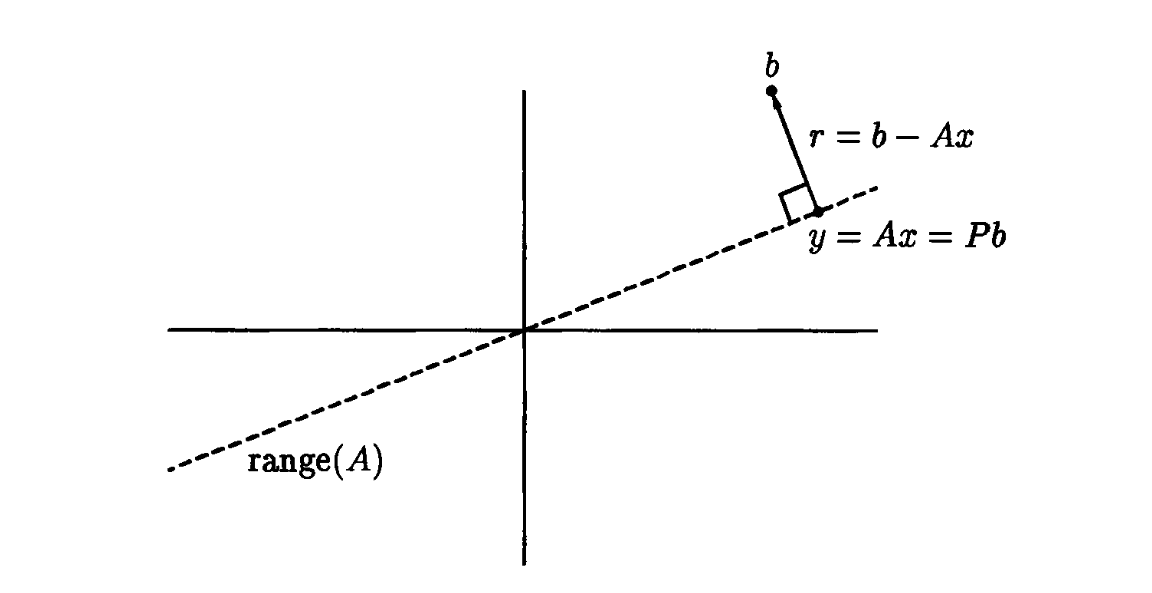
\includegraphics[width=0.8\textwidth]{figures/11-1.png}
    \label{fig 11.3} 
    \caption{Formulation of LS in terms of orthogonal projection}
\end{figure}
%────────────────────────────────────────

It is clear geometrically that this will occur provided $A x=P b$, where $P \in \mathbb{C}^{m \times m}$ is the orthogonal projector (Lecture 6) that maps $\mathbb{C}^m$ onto $\operatorname{range}(A)$. In other words, the residual $r=b-A x$ must be orthogonal to $\operatorname{range}(A)$. We formulate this condition as the following theorem.


%────────────────────────────────────────
\begin{theorem}
\label{thm: LS}
Let $A \in \mathbb{C}^{m \times n}(m \geq n)$ and $b \in \mathbb{C}^m$ be given. $A$ vector $x \in \mathbb{C}^n$ minimizes the residual norm $\|r\|_2=\|b-A x\|_2$, thereby solving the least squares problem \autoref{eq: least sq} if and only if $r \perp \operatorname{range}(A)$, that is,
$$
A^* r=0
$$
or equivalently,
\begin{equation}
    \label{eq: normal equations}
    A^* A x=A^* b
\end{equation}
or again equivalently,
$$
P b=A x,
$$
where $P \in \mathbb{C}^{m \times m}$ is the orthogonal projector onto range $(A)$. The $n \times n$ system of \autoref{eq: normal equations}, known as the \textbf{normal equations}, is nonsingular if and only if $A$ has full rank. Consequently the solution $x$ is unique if and only if $A$ has full rank.
\end{theorem}
%────────────────────────────────────────

\section{Pseudoinverse}


%────────────────────────────────────────
\begin{definition}
[Pseudoinverse]
\label{def: Pseudoinverse}
Given a full rank matrix $A$, the pseudoinverse of $A$ is 
\[
    A^\dagger =  (A^*A)^{-1}A^* \in \CC^{n\times m}. 
\]
\end{definition}
%────────────────────────────────────────
Hence, the LS problem is: 
\[
    x = A^\dagger b, \quad y = Pb. 
\]

\section{Normal Equations} 
Since $A^*A$ is Hermitian, the standard method of solving normal equations is by \textbf{Cholesky factorization}. This method constructs a factorization  $A^*A = R^*R$, where $R$ is upper-triangular. Hence, the equations are 
\[
    R^*R x = A^*b. 
\]
Here is the algorithm. 

\begin{algorithm}[H]
    \caption{Least Squares via Normal Equations}
    \label{Algo 11.1}
    Form the matrix $A^*A$ and the vector $A^*b$.\; 
    Compute the Cholesky factorization $A^*A = R^*R$.\; 
    Solve the lower-triangular system $R^*w = A^*b$ for $w$. \; 
    Solve the upper triangular system $Rx = w$ for $x$. 
\end{algorithm}

The steps that dominate the work for this computation are the first two (for steps 3 and 4, see Chapter 17). Because of symmetry, the computation of $A^* A$ requires only $m n^2$ flops, half what the cost would be if $A$ and $A^*$ were arbitrary matrices of the same dimensions. Cholesky factorization, which also exploits symmetry, requires $n^3 / 3$ flops. All together, solving least squares problems by the normal equations involves the following total operation count:


%────────────────────────────────────────
\begin{corollary}
\label{cor: cost of 11.1}
The work for \autoref{Algo 11.1}: $\sim m n^2+\frac{1}{3} n^3$ flops. 
\end{corollary}
%────────────────────────────────────────

\section{QR factorization} 
The "modern classical" method for solving least squares problems, popular since the 1960 s, is based upon reduced QR factorization. By Gram-Schmidt orthogonalization or, more usually, Householder triangularization, one constructs a factorization $A=\hat{Q} \hat{R}$. The orthogonal projector $P$ can then be written as $P= \hat Q \hat Q^*$.  Hence, 
\[
    y = Pb = \hat Q \hat Q^* b. 
\]
The system $Ax=y$ can be written as: 
\[
    \hat Q \hat R x = \hat Q \hat Q^* b\Rightarrow \hat R x = \hat Q^* b. 
\]

\begin{algorithm}[H]
    \caption{Least Squares via QR Factorization}
    \label{Algo 11.2}
    Compute the reduced QR factorization $A= \hat Q \hat R$\; 
    Compute the vector $\hat Q^* b$\; 
    Solve the upper-triangular system $\hat Rx = \hat Q^* b$ for x. 
\end{algorithm}

The work for \autoref{Algo 11.2} is dominated by the cost of QR. If we use Householder reflections, we have 

%────────────────────────────────────────
\begin{corollary}
\label{cor: Cost of algo 11.2}
Work for \autoref{Algo 11.2}: $ \sim 2 m n^2-\frac{2}{3} n^3 $ flops. 
\end{corollary}
%────────────────────────────────────────


\section{SVD}
In Chapter 31 we shall describe an algorithm for computing the reduced singular value decomposition $A = \hat U \hat \Sigma V^*$. Then $P= \hat U \hat U^*$, giving 
\[
    y = Pb = \hat U \hat U^* b, 
\]
and then 
\[
    \hat U \hat \Sigma V^* x = \hat U \hat U^* b \Rightarrow \hat \Sigma V^* x = \hat U^* b. 
\]
The algorithm is: 

\begin{algorithm}[H]
    \caption{Least Squares via SVD}
    \label{Algo 11.3}
    Compute the reduced SVD $A= \hat U \hat \Sigma V^*$\; 
    Compute the vector $\hat U ^* b$\; 
    Solve the diagonal system $\hat \Sigma w = \hat U^* b$ for $w$\; 
    Set $x= Vw$. 
\end{algorithm}

AS we shall see in Chapter 31, for $m\gg n$ this cost is approximately the same as for QR, but for $m\approx n$ the SVD is more expensive. 


%────────────────────────────────────────
\begin{corollary}
\label{cor: cost of SVD LS}
Work for \autoref{Algo 11.3}: $\sim 2mn^2 +11n^3 $ flops.  
\end{corollary}
%────────────────────────────────────────

\section{Comparison of Algorithms} 
Each of the methods we have described is advantageous in certain situations.
\begin{itemize}
    \item \autoref{Algo 11.1} is the fastest but solving the normal equations might not be stable; 
    \item Thus for many years, numerical analysts have recommended \autoref{Algo 11.2} instead as the standard method for least squares problems. This is indeed a natural and elegant algorithm, and we recommend it for ``daily use.''
    \item If A is close to rank-deficient, however, it turns out that \autoref{Algo 11.2} itself has less-than-ideal stability properties, and in such cases there are good reasons to turn to \autoref{Algo 11.3} based on the SVD.
\end{itemize}
